%\begin{multicols}{3}
\section{Results}
\lipsum
\begin{wrapfig}
	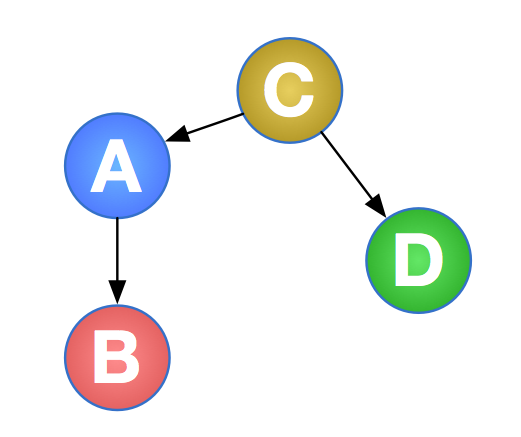
\includegraphics[width= \linewidth]{Resources/ABCD}%primer_tm_v}
	\captionof{figure}{Melting Temperatures (Tm) of Oligomeric DNA Fragments. (left) Melting Temperature against Fragment Length, color scale indicates Cytosine/Guanine Content, a black line indicates trend behaviour. (right) Melting Temperature against Cytosine/Guanine Content, color scale indicates fragment length.}
\end{wrapfig}
\subsection{Subresults}
\lipsum[4]

\begin{figure*}[t!]
	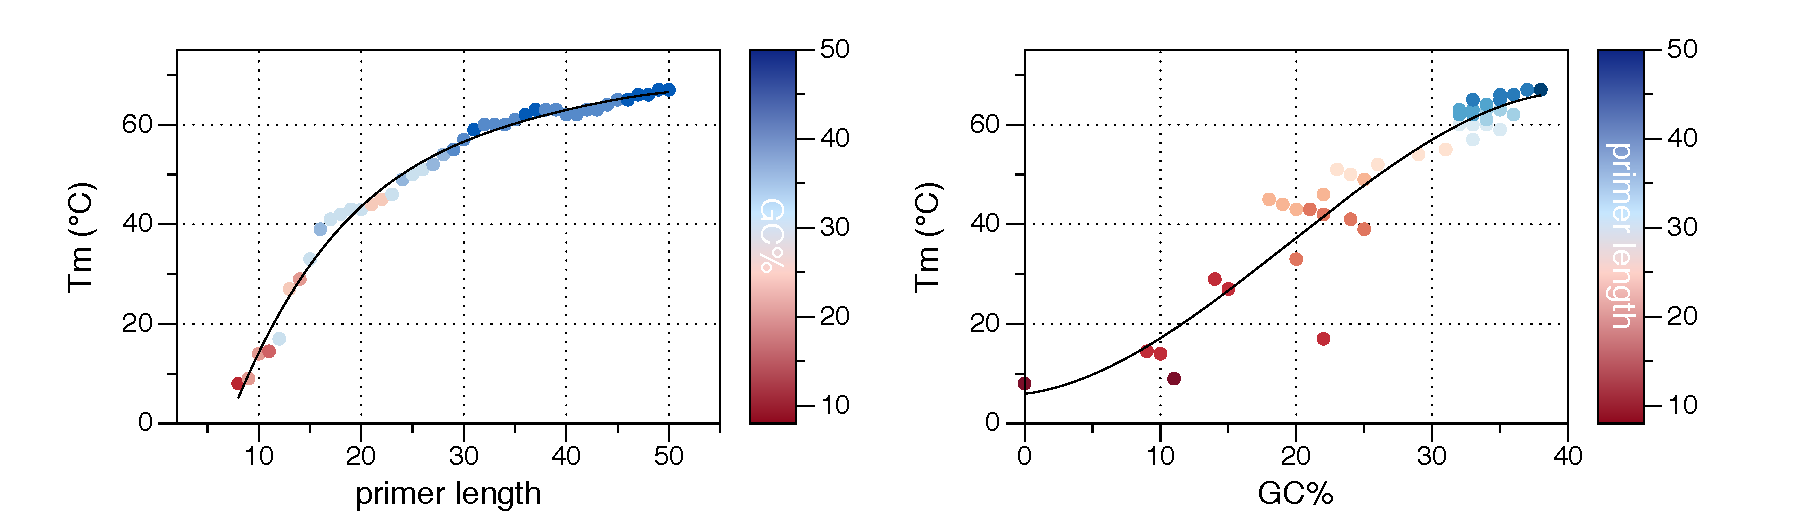
\includegraphics[width= \linewidth]{Resources/primer_tm_h}
	\captionof{figure}{Melting Temperatures (Tm) of Oligomeric DNA Fragments. (upper) Melting Temperature against Fragment Length, color scale indicates Cytosine/Guanine Content, a black line indicates trend behaviour. (lower) Melting Temperature against Cytosine/Guanine Content, color scale indicates fragment length.}
\end{figure*}
\lipsum



%\end{multicols}